\chapter{Testowanie Contiguous Memory Allocatora}

W~tym rozdziale opiszę jak przetestować alokator \acc{CMA} na
przykładzie laptopa U100 firmy \acc{MSI} z~jednym gibibajtem pamięci
\acc{RAM} działającym pod kontrolą systemem Slackware 14.0, który
można pobrać ze strony \href{http://slackware.com/}{\ttfamily
  slackware.com}.  Do testów wybrałem tę dystrybucję Linuksa, gdyż
jest stosunkowo prosta w~użyciu, a~jednocześnie pozostaje wierna
filozofii Uniksa, dzięki czemu łatwo jest wymieniać komponenty systemu
takie jak jego jądro.


\section{Instalacja jądra z~obsługą \acc{CMA}}

Domyślnie Linux nie posiada obsługi alokatora \acc{CMA}, dlatego
pierwszym krokiem będzie zmiana jądra systemu na wersję 3.5
z~włączonym mechanizmem \acc{CMA}.  Wymagane źródła można pobrać ze
strony \href{http://kernel.org/}{\ttfamily kernel.org}, która jest
głównym miejscem dystrybucji Linuksa.

Przed kompilacją jądra należy je najpierw skonfigurować wybierając,
które funkcje i~sterowniki mają być dostępne.  Aby ułatwić ten proces,
zamiast ustawiać wszystkie opcje od początku, warto skorzystać z~już
istniejącego pliku konfiguracyjnego.  Zazwyczaj jest on dostępny
w~skompresowanej formie jako plik
\code{/proc/config.gz}\footnote{W~dystrybucjach innych niż Slackware
  plik ten może byc nieobecny.  W~takim przypadku należy sprawdzić
  obecność pliku \code{/proc/config}.  Jeżeli również i~ten plik nie
  jest dostępny, warto poszukać plików których nazwa rozpoczyna się od
  \code{config} w~katalogu \code{/boot}.}.  Aby pobrać źródła Linuksa,
a~następnie włączyć program konfiguracji, należy wykonać następującą
sekwencję poleceń:

\begin{lstlisting}[language=sh,numbers=none,columns=fullflexible]
wget http://www.kernel.org/pub/linux/kernel/v3.0/linux-3.5.tar.xz
xz -d <linux-3.5.tar.xz | tar xf
cd linux-3.5
gzip -d </proc/config.gz >.config
make xconfig
\end{lstlisting}

Uruchomi to aplikację graficzną (opartą o~bibliotekę Qt), która
pozwala wybrać opcje z~jakimi jądro ma zostać zbudowane.  W~przypadku
kompilacji w~środowisku tekstowym, zamiast polecenia
\code{make xconfig} należy wykonać komendę \code{make menuconfig}, która
uruchomi interfejs oparty o~bibliotekę ncurses.

Aby móc testować \acc{CMA} należy w~programie konfiguracyjnym jądra
zaznaczyć opcje \ang*{Prompt for development and/or incomplete
  code/drivers} w~sekcji \ang*{General setup}
(zob.\ rys.\ \subref*{fig:xconfig-exp}) oraz \ang*{Contiguous Memory
  Allocator} w~sekcji \ang*{Device Drivers $\rightarrow$ Generic
  Driver Options} (zob.\ rys.\ \subref*{fig:xconfig-cma}).  Ponadto,
aby umożliwić dalsze testy należy również upewnić się, że wybrana jest
opcja \ang*{Enable loadable module support}\,---\,bez niej nie będzie
możliwe zbudowanie ani załadowanie modułu testowego opisanego
w~następnym podrozdziale.

\begin{figure}[tbp]
  \centering
  \subfloat[Opcja umożliwiająca wybór eksperymentalnych funkcji jądra.]{
    \label{fig:xconfig-exp}
    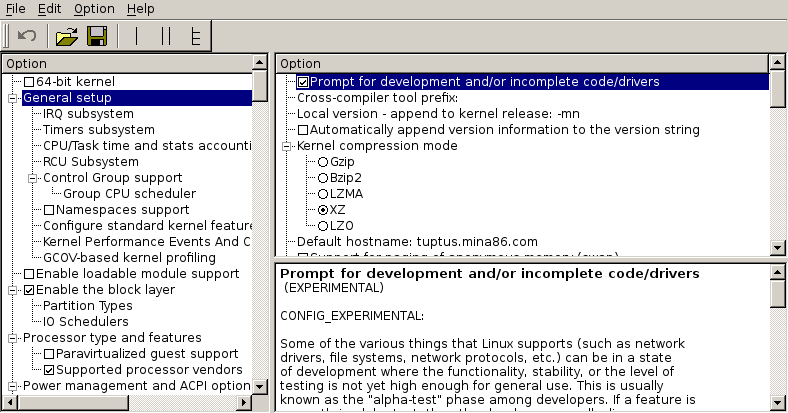
\includegraphics[width=.9\textwidth]{build/xconfig-exp.eps}
  }
  \vspace{\baselineskip}
  \subfloat[Opcja włączająca \acc{CMA}.]{
    \label{fig:xconfig-cma}
    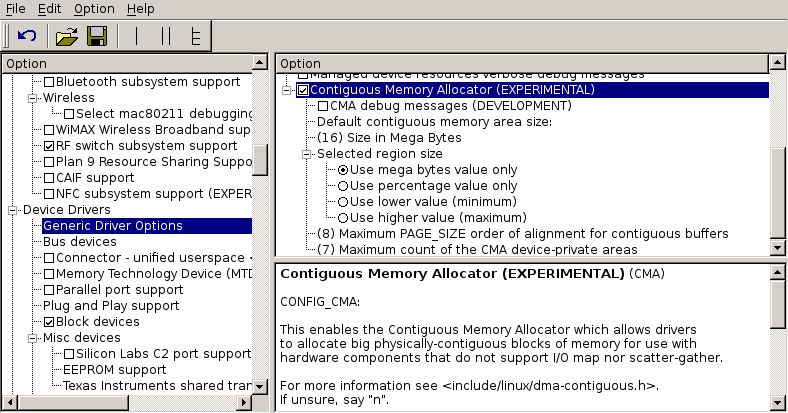
\includegraphics[width=.9\textwidth]{build/xconfig-cma.eps}
  }
  \caption{Graficzny interfejs konfiguracji jądra.}
  \label{fig:xconfig}
\end{figure}

W~przypadku jakichkolwiek problemów ze znalezieniem danej opcji, warto
skorzystać z~funkcji wyszukiwania wbudowanej w~program konfiguracyjny.
Aktywuje się ją wciśnięciem sekwencji klawiszy Ctrl+F (lub w~przypadku
tekstowego interfejsu \code{menuconfig} poprzez wciśnięcie ukośnika).

Po zakończeniu konfiguracji należy zbudować i~zainstalować nowe jądro
zgodnie z~opisem w~\autocite{bib:building-linux}.  Do testów alokatora
\acc{CMA} warto ponadto stworzyć dodatkowe trzy wpisy w~pliku
\code{/etc/lilo.conf} różniące się opcją \code{append}, które
instruuje program startujący \acc{LILO}, aby przekazał dodatkowe
argumenty do jądra:

\begin{enumerate}
\item \code{append = " cma=0"}
\item \code{append = " cma=0 mem=512m"}
\item \code{append = " cma=512m"}
\end{enumerate}

Pierwsza i~druga opcja wyłączy \acc{CMA} tak, że jądro będzie
zachowywać się jakby obsługa \acc{CMA} nie była dostępna.  Druga opcja
dodatkowo spowoduje, że Linux będzie korzystał tylko z~pierwszych
\unit[512]{MiB} pamięci \acc{RAM}.  Pozwala to symulować sytuację,
w~której część pamięci jest na stałe zarezerwowane dla sterowników.
Ostatnia opcja poinstruuje alokator \acc{CMA}, by zarezerwował
pojedynczy region rozmiaru \unit[512]{MiB} do wykorzystania dla
sterowników.  Wszystkie te trzy opcje są wykorzystywane w~testach
opisanych w~tym rozdziale.

Po wystartowaniu systemu z~nowym jądrem, obecność mechanizmu \acc{CMA}
można sprawdzić analizując plik \code{/proc/pagetypeinfo}.  Zawiera on
statystyki alokatora stron w~postaci liczby stron różnych typów
w~poszczególnych strefach.  Jeżeli alokator \acc{CMA} jest obecny
w~jądrze plik ten posiada linie zawierające nazwę \code{CMA}, które
informują ile stron \acc{CMA} jest wolnych w~systemie.  Ponadto plik
\code{/proc/cmdline} zawiera pełną listę argumentów jakie program
startujący przekazał jądru.  Może on być przydatny do weryfikacji, czy
opcje są poprawnie przekazywane.


\section{Modułu \code|cma_test|}

Do testów \acc{CMA} wykorzystam moduł Barry'ego Songa.  Po nałożeniu
\autocite{patch:cma-test} na źródła jądra powstanie katalog
\code{tools/cma} z~nowym sterownikiem.  Niestety był on testowany
jedynie na architekturze \acc{ARM} i~aby zadziałał na systemie x86
należy zmodyfikować plik \code{cma_test.c} wprowadzając dwie zmiany.
Po pierwsze, zaraz po ostatniej dyrektywie \code{#include} należy
dodać następujące linie:

\begin{lstlisting}[numbers=none]
#ifndef SZ_1K
#  define SZ_1K 1024
#endif

static u64 cma_test_dma_mask = ~(u64)0;
\end{lstlisting}

Po wtóre, w~funkcji \code{cma_test_init}, tuż przed linią przypisującą
wartość do pola \code{coherent_dma_mask} obiektu \code{cma_dev},
należy dodać linijkę:

\begin{lstlisting}[numbers=none]
	cma_dev->dma_mask = &cma_test_dma_mask;
\end{lstlisting}

Po wprowadzeniu tych modyfikacji moduł można skompilować wykonując
polecenie \code{make} wewnątrz katalogu \code{tools/cma}, w~wyniku
czego powstanie plik \code{cma_test.ko}.  Całą operację (łącznie
z~pobieraniem i~dodaniem źródeł modułu do jądra) można sprowadzić do
wykonania sekwencji poleceń z~wydruku \ref{lst:compile-cma-test}
w~katalogu ze źródłami Linuksa.

\begin{lstlisting}[float=tb,caption=Sekwencja komend dodająca
    i~budująca moduł \code{cma_test}.,label=lst:compile-cma-test,
    language=sh,numbers=none,columns=fullflexible]
wget -O cma_test.patch https://patchwork.kernel.org/patch/1158071/raw/
patch -p1 <cma_test.patch
cd tools/cma
sed -i -e '/struct cma_allocation {/ i\
#ifndef SZ_1K\
#  define SZ_1K 1024\
#endif\
\
static u64 cma_test_dma_mask = ~(u64)0;\
\
/coherent_dma_mask/ i	cma_dev->dma_mask = &cma_test_dma_mask;' cma_test.c
make
\end{lstlisting}

Po wczytaniu modułu poleceniem \code{insmod cma_test.ko} w~systemie
pojawi się urządzenie \code{/dev/cma_test}, które służy do wykonywania
testowych alokacji z~wykorzystaniem interfejsu \acc{DMA} \acc{API}
(a~zatem pośrednio z~użyciem alokatora \acc{CMA}).  Zapis do tego
pliku liczby naturalnej spowoduje wykonanie alokacji podanej liczby
kibibajtów, a~odczyt zwolnienie najwcześniej zaalokowanego obszaru.

Przykładowo wykonanie polecenia \code{echo 10240 >/dev/cma_test}
spowoduje alokację bufora o~rozmiarze \unit[10]{MiB}, gdy tymczasem
polecenie \code{cat /dev/cma_test} spowoduje zwolnienie tego obszaru.


\section{Testowanie alokacji pamięci}

Aby zobaczyć efekt działania opcji \code{mem} oraz mechanizmu
\acc{CMA} wykorzystać można prosty program \code{malloc} przedstawiony
na wydruku \ref{lst:malloc}.  Nie robi on nic poza żądaniem pamięci
w~pętli.  Linux domyślnie opóźnia alokację pamięci do pierwszej próby
modyfikacji buforu, dlatego program musi zapisać coś w~zaalokowanej
stronie.

\lstinputlisting[float=tb,caption=Prosty program testujący alokację
  pamięci.,label=lst:malloc]{code/malloc.c}

Po uruchomieniu program będzie działał w~kółko żądając coraz więcej
pamięci do momentu, gdy jądro nie będzie już w~stanie zaspokoić tych
żądań.  Wówczas \ang*{out-of-memory killer} wymusi zakończenie
programu.  Jest to mechanizm jądra, którego celem jest
zagwarantowanie, że system zawsze będzie miał pewne rezerwy wolnej
pamięci.

Uruchomiony na systemie z~jednym gibibajtem pamięci program zakończył
się po zaalokowaniu około \unit[965]{MiB}, gdy mechanizm \acc{CMA} był
wyłączony, oraz \unit[964]{MiB}, gdy na potrzeby \acc{CMA} było
zarezerwowane \unit[512]{MiB}.  Różnica jednego mebibajta jest
pomijalna i~wskazuje, iż istotnie pamięć rezerwowana przez \acc{CMA}
jest dostępna dla systemu.

Jednocześnie gdy system uruchomiono z~opcją \code{mem=512m}, program
został zatrzymany po zaalokowaniu zaledwie
\unit[477]{MiB}\,---\,pokazuje to w~praktyce działanie argumentu
\code{mem} jądra.  Podobnie gdy system wystartował z~regionem
\acc{CMA} o~rozmiarze \unit[512]{MiB}, a~następnie dokonano alokacji
tej pamięci poprzez czterokrotne wykonanie polecenia
\code{echo 131072 >/dev/cma_test}, program \code{malloc} nie był
w~stanie zaalokować więcej niż \unit[454]{MiB} pamięci.  Spowodowane
to było rzecz jasna tym, iż sterownik \code{cma_test} trzymał połowę
pamięci i~jądro miało do dyspozycji jedynie \unit[512]{MiB}.

Ilość pamięci, którą udało się zaalokować programowi \code|malloc|
przy różnych ustawieniach jądra oraz różnych buforach zaalokowanych
z~puli \acc{CMA} przedstawia tablica \ref{tab:cma-test-allocs}.
Kolumna „\code|append|” tej tablicy określa parametry przekazane do
jądra, kolumna „Alokacja \acc{CMA}” określa jaki rozmiar pamięci
\acc{CMA} został zaalokowany przez moduł testowy \code{cma_test},
a~kolumna „Udana alokacja” wskazuje ile pamięci udało się zaalokować
programowi \code{malloc} zanim system wymusił jego zakończenie.

\begin{table}[tbp]
\begin{center}
\begin{tabular}{llrr}
    & \code|append|         & Alokacja \acc{CMA} & Udana alokacja \\
\hline
(1) & \code|cma=0|          &                   & \unit[965]{MiB} \\ % 988284
(2) & \code|cma=512m|       &     \unit[0]{MiB} & \unit[964]{MiB} \\ % 987628
(3) & \code|cma=512m|       &   \unit[128]{MiB} & \unit[837]{MiB} \\ % 857428
(4) & \code|cma=512m|       &   \unit[256]{MiB} & \unit[710]{MiB} \\ % 726804
(5) & \code|cma=512m|       &   \unit[384]{MiB} & \unit[582]{MiB} \\ % 596108
(8) & \code|cma=512m|       &   \unit[512]{MiB} & \unit[455]{MiB} \\ % 465420
(7) & \multicolumn{2}{l}{\code|cma=0 mem=512m|} & \unit[477]{MiB} \\ % 488900
\end{tabular}
\end{center}
\caption[Ilość zaalokowanej z~sukcesem pamięci.]{Ilość pamięci
  zaalokowanej z~sukcesem na testowym systemie z~jednym \unit{GiB}
  pamięci.}
\label{tab:cma-test-allocs}
\end{table}


\section{Testowanie szybkości działania systemu}

Aby zmierzyć jak zmniejszona ilość dostępnej pamięci może wpływać na
szybkość systemu posłużę się programem \code{seq_read} zaprezentowanym
na wydruku \ref{lst:seq-read}.  Jego działanie sprowadza się do
sekwencyjnego odczytu podanego pliku\footnote{Należy zauważyc, że
  program odczytuje jedynie pierwszy bajt z~każdych \unit[4]{KiB}
  zadanego pliku.  Ponieważ wykorzystana jest funkcja \code|mmap|
  wymusza to wczytanie całego bloku do pamięci, jednak jeżeli strona
  posiada już potrzebne dane, odczyt jest szybszy niż odczyt całej
  strony z~pamięci RAM.  Program \code|seq_read| jest napisany w~ten
  sposób, aby uwypuklić efekty buforowania.} i przyjmuje trzy
argumenty:

\begin{enumerate}
\item Nazwę pliku, który ma być odczytany.  Musi to być zwykły plik,
  którego rozmiar jest nie mniejszy niż jedna strona (\unit[4096]{B}).
\item Opcionalną liczbę określającą ile razy plik ma być odczytany.
  Wielokrotny odczyt pozwala z~większą dokładnością zmierzyć ile czasu
  zajmuje pojedynczy odczyt.  Jeżeli argument ten nie jest podany,
  plik zostanie odczytany tylko raz.
\item Opcjonalną liczbę określającą maksymalny rozmiar pliku.  Jeżeli
  argument jest podany i~jest mniejszy od rozmiaru pliku, tylko podana
  liczba bajtów będzie brana pod uwagę.  Pozwala to testować różne
  rozmiary plików stosując tylko jeden duży plik.
\end{enumerate}

\lstinputlisting[float=p,caption=Prosty program sekwencyjnie
    odczytujący plik.,label=lst:seq-read]{code/seq_read.c}

Przeprowadzone przeze mnie testy polegały na zmierzeniu ile czasu
zajmie programowi \code|seq_read| odczyt pliku najpierw raz, a~potem
sto razy.  Oba wywołania programu wykonałem dla różnych wartości
argumentu \code|append| oraz z~różnym rozmiarem zaalokowanych buforów
\acc{CMA}, za każdym razem restartując system.  Do zautomatyzowania
tego procesu, posłużyłem się skryptem \code|run_test.sh|
przedstawionym na wydruku \ref{lst:run-test}.  Do poprawnego działania
wymaga on obecności pliku \code|rand| o~rozmiarze przynajmniej
\unit[900]{MiB}, który można stworzyć za pomocą następującej sekwencji
poleceń:

\begin{lstlisting}[language=sh,numbers=none,columns=fullflexible]
head -c 900 /dev/urandom >rand
for i in $(seq 20); do cat rand rand >tmp && mv tmp rand; done
\end{lstlisting}

Pierwsze dwa argumenty skryptu \code|run_test.sh| mają takie samo
znaczenie jak drugi i~trzeci argument programu \code|seq_read|, tyle
że maksymalna wielkość podana jest w~mebibajtach, a~nie w~bajtach.
Ponadto, trzeci argument, jeżeli jest podany, określa ile bloków
rozmiaru \unit[128]{MiB} ma być zaalokowanych przez moduł
\code|cma_test| przed uruchomieniem testów.  Aby ta opcja działała
poprawnie program musi być uruchomiany z~konta użytkownika \code|root|
oraz moduł \code|cma_test| musi być wczytany albo plik
\code|cma_test.ko| dostępny.

Dzięki uruchomieniu programu \code|seq_read| poprzez polecenie
\code|time|, automatycznie następuje pomiar czasu.  Po zakończeniu obu
wywołań programu \code|seq_read| skrypt \code|run_test.sh| czeka na
wciśnięcie klawisza Enter, po czym restartuje system (aby temu
zapobiec, wystarczy zamiast Enter wcisnąć Ctrl+D).

\lstinputlisting[float=tb,caption=Skrypt \code|run_test.sh| służący do
  wykonywania pojedynczej iteracji testu.,columns=fullflexible,
  label=lst:run-test,language=sh]{code/run_test.sh}

Tablica \subref*{tab:seq-read-times-first} przedstawia czas jaki był
potrzebny do jednorazowego odczytania zadanej liczby mebibajtów pliku.
Zgodnie z~przewidywaniami, ponieważ zaraz po uruchomieniu komputera
system nie miał szansy buforować pliku, liczba dostępnej pamięci nie
wpływa na czas działania programu\,---\,za każdym razem jądro musi
bowiem wczytać cały plik.

O~wiele ciekawsza jest tablica \subref*{tab:seq-read-times-nth:sub},
która pokazuje ile czasu zajął pojedynczy odczyt po zakończeniu
wstępnego odczytu.  W~przypadku, gdy w~systemie jest dużo wolnej
pamięci, jądro jest w~stanie trzymać cały plik w~pamięci, dzięki czemu
kolejne odczyty są bardzo szybkie i~nawet odwołanie się do
\unit[900]{MiB} zajmuje niecałe cztery setne sekundy.

\begin{table}[tbp]
  \centering
  \subfloat[Czas potrzebny do odczytania podanej liczby mebibajtów
    pliku zaraz po restarcie systemu, zatem gdy bufory dyskowe nie
    zawierają żadnych danych.]{
    \label{tab:seq-read-times-first}
    \begin{tabular}{llrrrr}
    & & & \multicolumn{3}{c}{Czas pierwszego odczytu} \\
    & \code|append|        & Alokacja \acc{CMA} & \unit[300]{MiB} & \unit[600]{MiB}  & \unit[900]{MiB}  \\
\hline
(1) & \code|cma=0|            &                 & \unit[5,925]{s} & \unit[11,598]{s} & \unit[17,426]{s} \\
(2) & \code|cma=512m|         &   \unit[0]{MiB} & \unit[5,839]{s} & \unit[11,685]{s} & \unit[17,537]{s} \\
(3) & \code|cma=512m|         & \unit[128]{MiB} & \unit[5,844]{s} & \unit[11,798]{s} & \unit[17,554]{s} \\
(4) & \code|cma=512m|         & \unit[256]{MiB} & \unit[5,803]{s} & \unit[11,701]{s} & \unit[17,645]{s} \\
(5) & \code|cma=512m|         & \unit[384]{MiB} & \unit[5,764]{s} & \unit[11,726]{s} & \unit[17,456]{s} \\
(6) & \code|cma=512m|         & \unit[512]{MiB} & \unit[5,885]{s} & \unit[11,773]{s} & \unit[17,449]{s} \\
(7) & \multicolumn{2}{l}{\code|cma=0 mem=512m|} & \unit[5,701]{s} & \unit[11,784]{s} & \unit[17,627]{s} \\
    \end{tabular}
  }
  \vspace{\baselineskip}
  \subfloat[Czas potrzebny do odczytania podanej liczby mebibajtów
    pliku, gdy dane już były raz odczytane i~potencjalnie znajdują się
    w~buforach dyskowych.]{
    \label{tab:seq-read-times-nth:sub}
    \begin{tabular}{llrrrr}
    & & & \multicolumn{3}{c}{Czas kolejnych odczytów} \\
    & \code|append|        & Alokacja \acc{CMA} & \unit[300]{MiB} & \unit[600]{MiB}  & \unit[900]{MiB}  \\
\hline
(1) & \code|cma=0|            &                 & \unit[0,011]{s} & \unit[ 0,023]{s} & \unit[ 0,035]{s} \\
(2) & \code|cma=512m|         &   \unit[0]{MiB} & \unit[0,011]{s} & \unit[ 0,024]{s} & \unit[ 0,037]{s} \\
(3) & \code|cma=512m|         & \unit[128]{MiB} & \unit[0,012]{s} & \unit[ 0,029]{s} & \unit[17,117]{s} \\
(4) & \code|cma=512m|         & \unit[256]{MiB} & \unit[0,011]{s} & \unit[ 0,024]{s} & \unit[16,941]{s} \\
(5) & \code|cma=512m|         & \unit[384]{MiB} & \unit[0,012]{s} & \unit[ 9,211]{s} & \unit[17,094]{s} \\
(6) & \code|cma=512m|         & \unit[512]{MiB} & \unit[0,012]{s} & \unit[11,633]{s} & \unit[17,382]{s} \\
(7) & \multicolumn{2}{l}{\code|cma=0 mem=512m|} & \unit[0,012]{s} & \unit[11,640]{s} & \unit[17,368]{s} \\
    \end{tabular}
  }
  \vspace{\baselineskip}
  \subfloat[Graficzna reprezentacja danych z~tablicy
    \subref{tab:seq-read-times-nth:sub}.  Oś y jest w~skali
    logarytmicznej.  Numery na osi x~odpowiadają wierszom tablicy.]{
    \label{fig:seq-read-times-nth}
    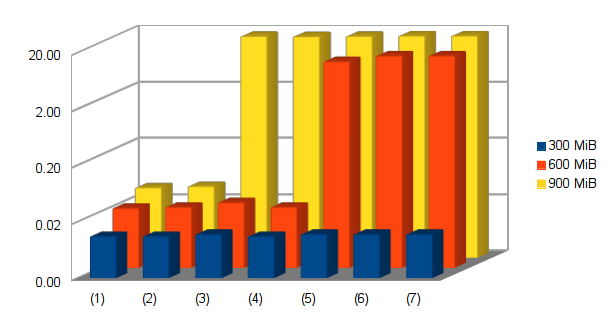
\includegraphics[width=.9\textwidth]{build/seq-read-times.eps}
  }
  \caption[Czas odczytu pliku, gdy dane były już raz odczytane.]{}
\label{tab:seq-read-times-nth}
\end{table}

Gdy ilość pamięci, którą system może przeznaczyć na bufory dyskowe
maleje, czas odczytu gwałtownie rośnie.  Gdy zaledwie \unit[128]{MiB}
zostanie zaalokowanych przy użyciu mechanizmu \acc{CMA} (wiersz (3)
tablicy \ref{tab:seq-read-times-nth}), czas potrzebny do odczyt
\unit[900]{MiB} „skacze” do około \unit[17]{s}, czyli czasu podobnego
do tego potrzebnego do odczytu pliku „na zimno”.  Wynika to z~faktu,
że kolejne odczytywane strony „wyrzucają” z~pamięci wcześniejsze
strony pliku przez co, gdy program ponownie zaczyna odczytywać plik od
początku, dane nie znajdują się już w~pamięci.

Również ciekawe jest zachowanie systemu, gdy moduł \code|cma_test|
zaalokuje \unit[384]{MiB}.  Jak wynika z~wiersza (5) tablicy
\ref{tab:cma-test-allocs} jądro może wówczas przeznaczyć około
\unit[582]{MiB} na bufory dyskowe.  Jest to rozmiar na tyle bliski
\unit[600]{MiB}, że przy odczycie właśnie takiego pliku widać poprawę
w~stosunku do sytuacji, gdy \unit[512]{MiB} jest zarezerwowanych przez
\acc{CMA}, niemniej „brakujące” \unit[12]{MiB} znacznie spowalnia
program \code|seq_read| z~tych samych powodów co opisane powyżej.


\section{Podsumowanie}

Testy szybkości odczytu pliku pokazują w~jak dużym stopniu brak wolnej
pamięci może spowolnić pracę systemu.  Co prawda odczyt w~kółko
pojedynczego pliku nie jest realnym scenariuszem działania prawdziwego
programu, niemniej aplikacje bazodanowe, czy oprogramowanie do obróbki
multimediów często charakteryzują się losowym dostępem do dysku.  Przy
niewielkiej ilości wolnej pamięci, tego typu programy będą cierpiały
na te same problemy co aplikacja \code|seq_read|.

Pokazuje to jak istotne jest, że alokator \acc{CMA} spełnia swoje
założenia i~pozwala sterownikom alokować duże obszary ciągłej
fizycznie pamięci, a~jednocześnie udostępnia zarezerwowaną pamięć
jądru podczas, gdy nie jest ona wykorzystywana przez żadne urządzenie.
To właśnie ta cecha mechanizmu \acc{CMA} odróżnia go od innych
rozwiązań problemu alokacji ciągłych fizycznie obszarów pamięci.
